\section{Results and Performance Evaluation}
\label{sec:rpe}

Let's now analyse the results achieved from every kinematic inversion, then a comparison among these will be performed. The computation time of every kinematics inversion has been recorded with the Matlab \textit{tic-toc} system. 
The computed trajectory has 10 points per segment for falling and rising phases, since distance travelled is lower, and 70 point for each segment of the polygon, so total dimension is 300 points.

\subsection{Linear Inverse Kinematics Results}

As one could expect errors are very low since all values are computed directly and only numerical approximations could create some drift from desired values. The computation time is 0.79 seconds, the magnitude order of such value would be clearer once compared with others.
\begin{figure}[ht]
	\centering
	\subfloat[x-axes error]{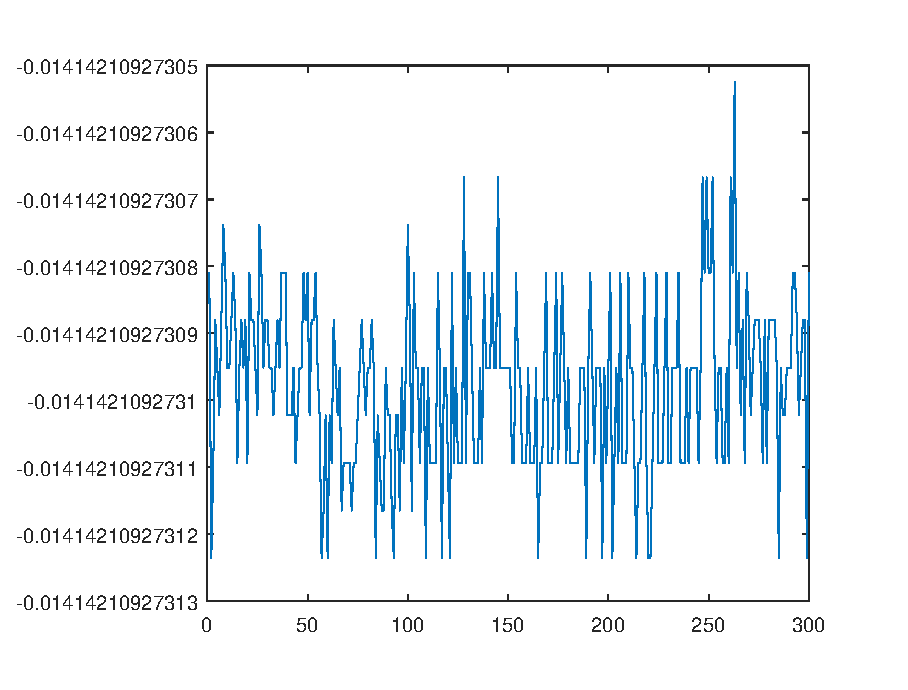
\includegraphics[width=0.5\linewidth]{img/xaxerlik}}
	\subfloat[y-axes error]{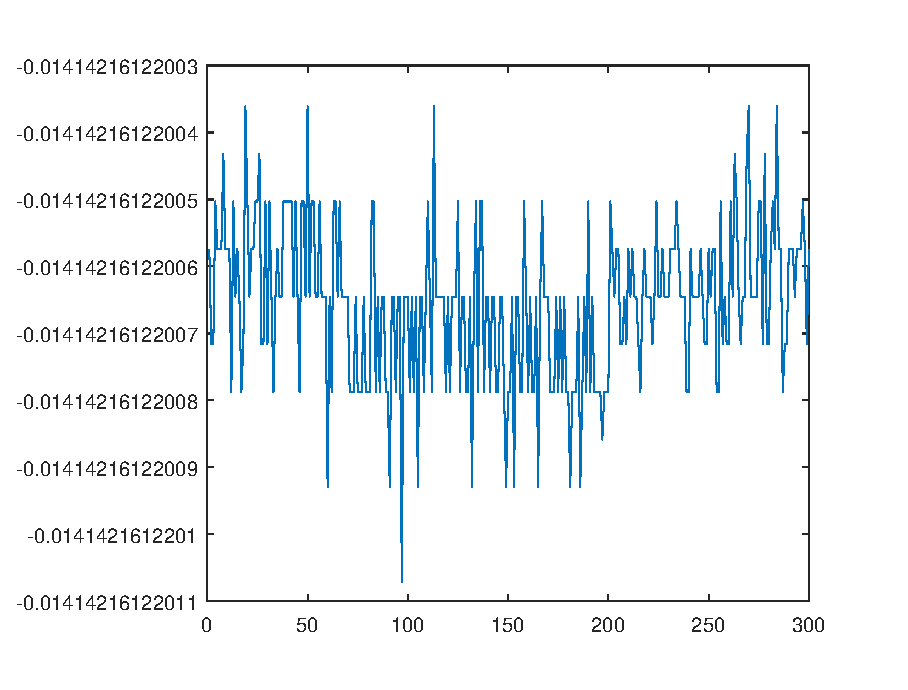
\includegraphics[width=0.5\linewidth]{img/yaxerlik}}
	\hspace{1cm}
	\subfloat[z-axes error]{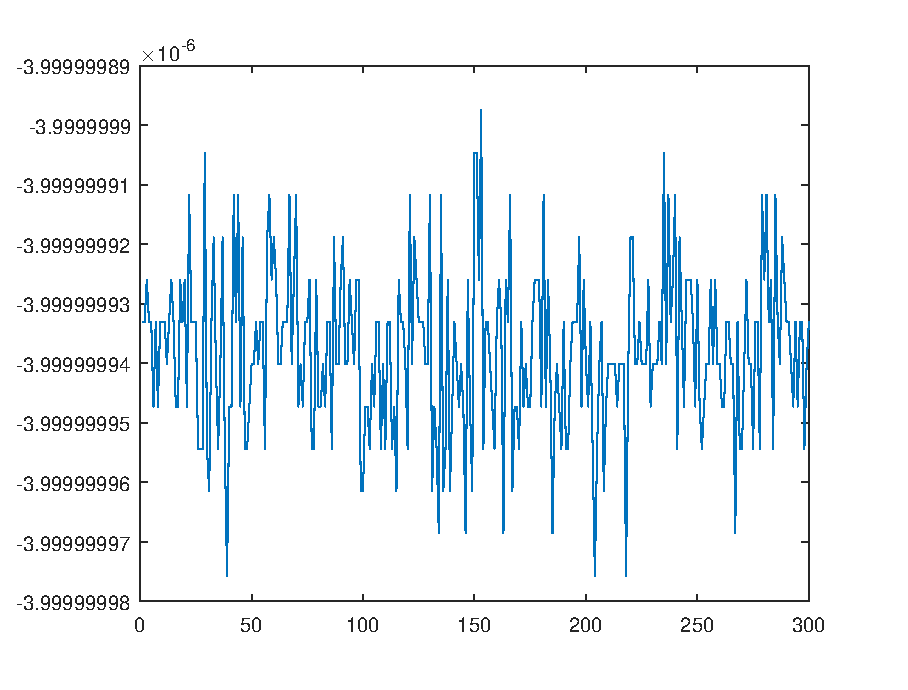
\includegraphics[width=0.5\linewidth]{img/zaxerlik}}
	\subfloat[Roll-Angle error]{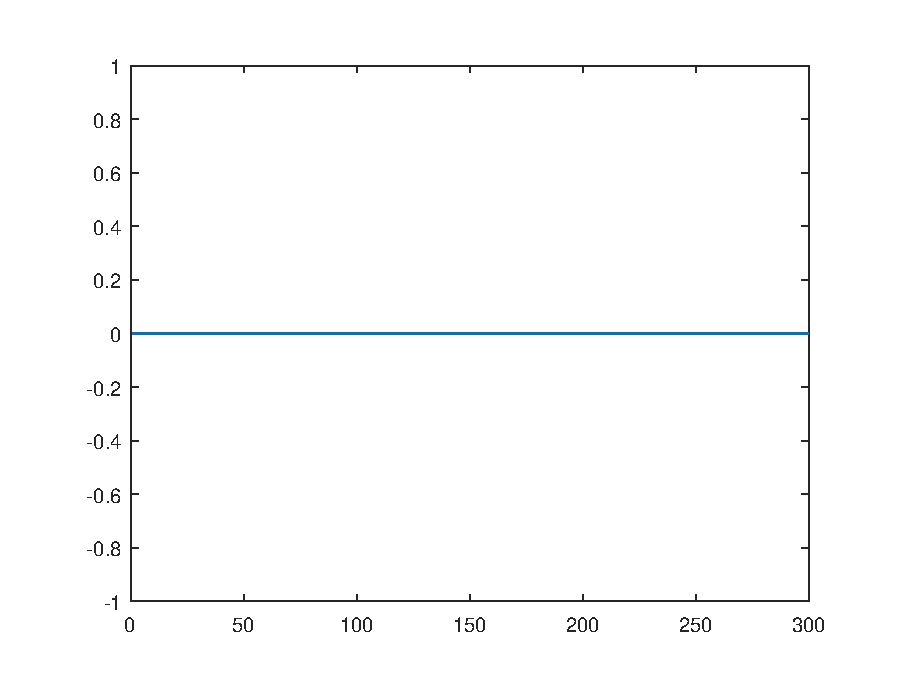
\includegraphics[width=0.5\linewidth]{img/rerlik}}
\end{figure}
\clearpage
\begin{figure}[!t]
	\centering
	\subfloat[{Pitch-Angle error}]{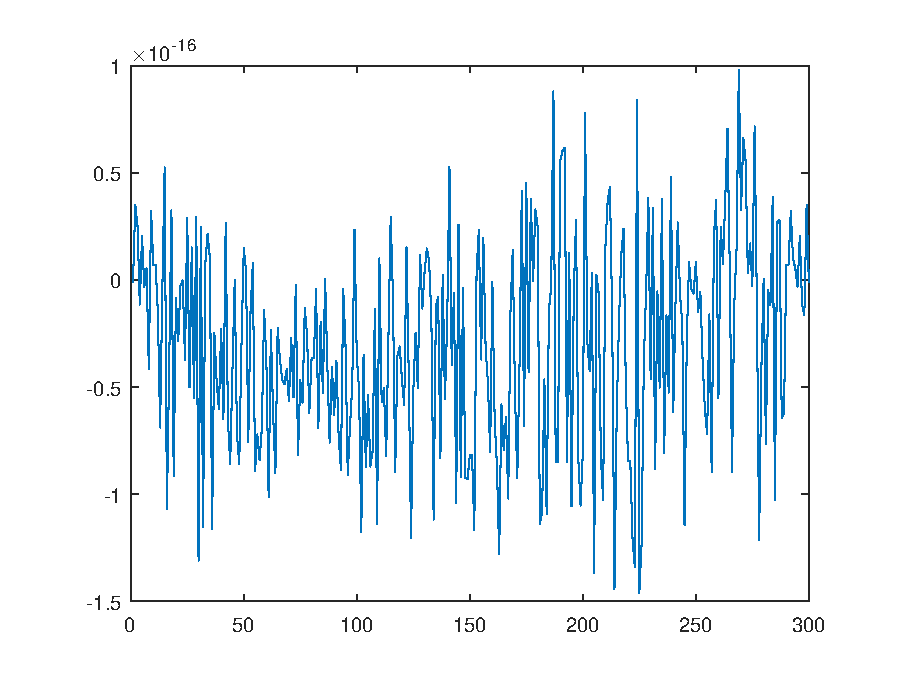
\includegraphics[width=0.5\linewidth]{img/perlik}}
	\subfloat[Manipulability]{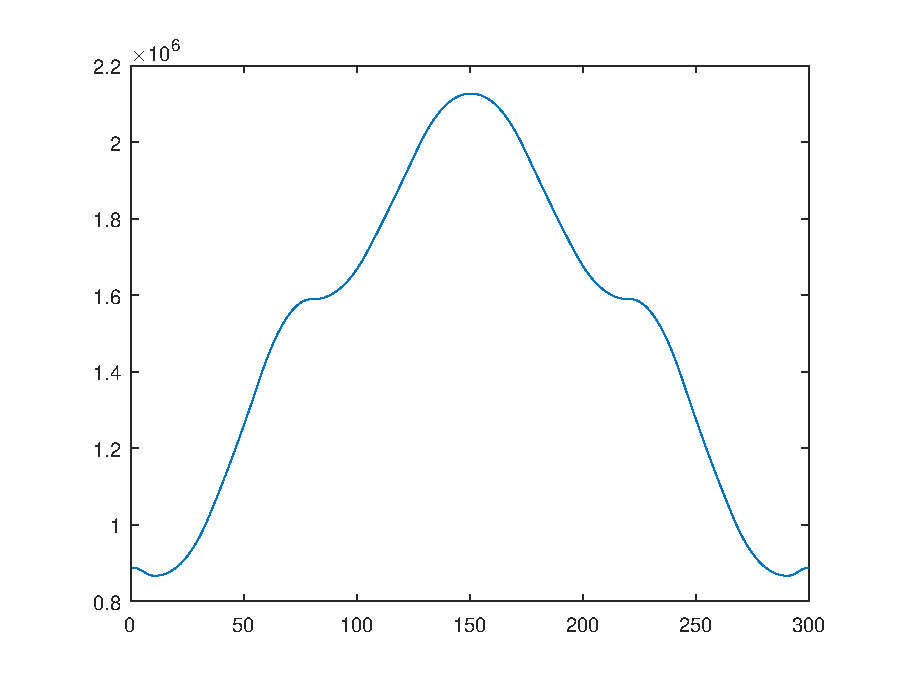
\includegraphics[width=0.5\linewidth]{img/manlik}}
	\hspace{1cm}
	\subfloat[Joint Trajectory]{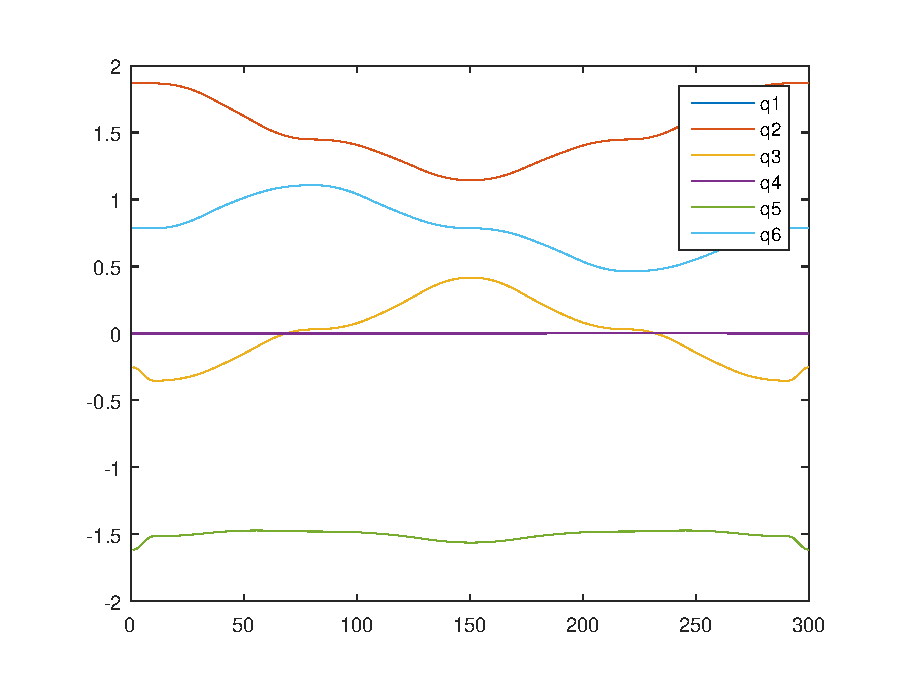
\includegraphics[width=0.7\linewidth]{img/jolik}}
\end{figure}

\subsection{Differential Kinematics Inversion}
\label{ssec:dikres}

At this stage the pose-error significantly increases since the kinematics inversion is performed in open-loop and numerical integration error is involved. It is worth to notice that the orientation error, even if it increases about 12 order magnitude with respect to the previous, remain reasonably low, indeed such error could be only visible in manipulators with resolution less or equal to $10^{-4}$, i.e tenths of millimetres. Computation time is 0.5242 seconds, quite similar to linear inversion.
\begin{figure}
	\label{fig:dikerr}
	\centering
	\subfloat[x-axes error]{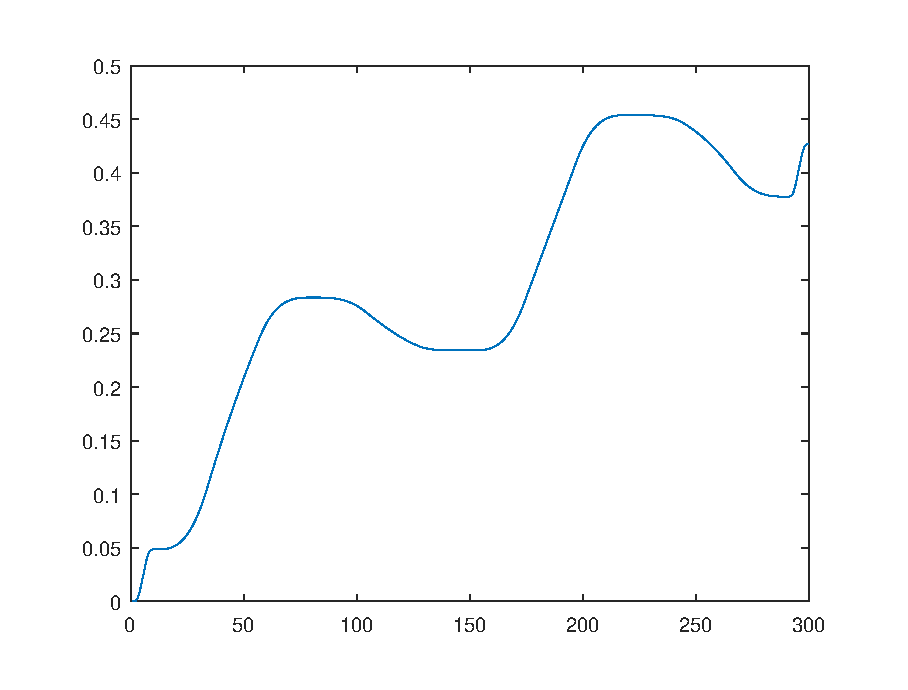
\includegraphics[width=0.5\linewidth]{img/xaxerdik}}
	\subfloat[y-axes error]{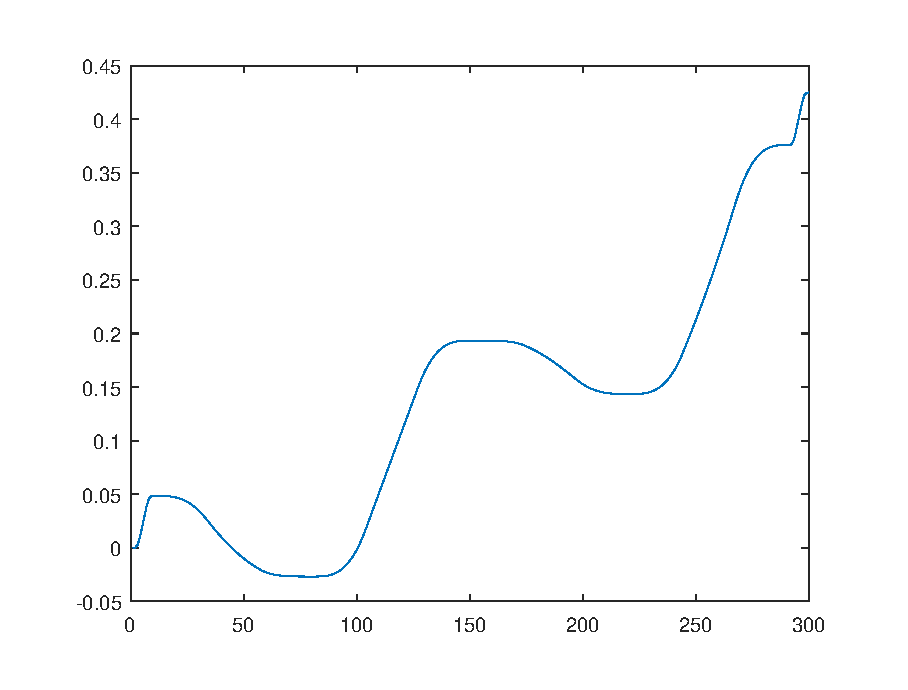
\includegraphics[width=0.5\linewidth]{img/yaxerdik}}
	\hspace{1cm}
	\subfloat[z-axes error]{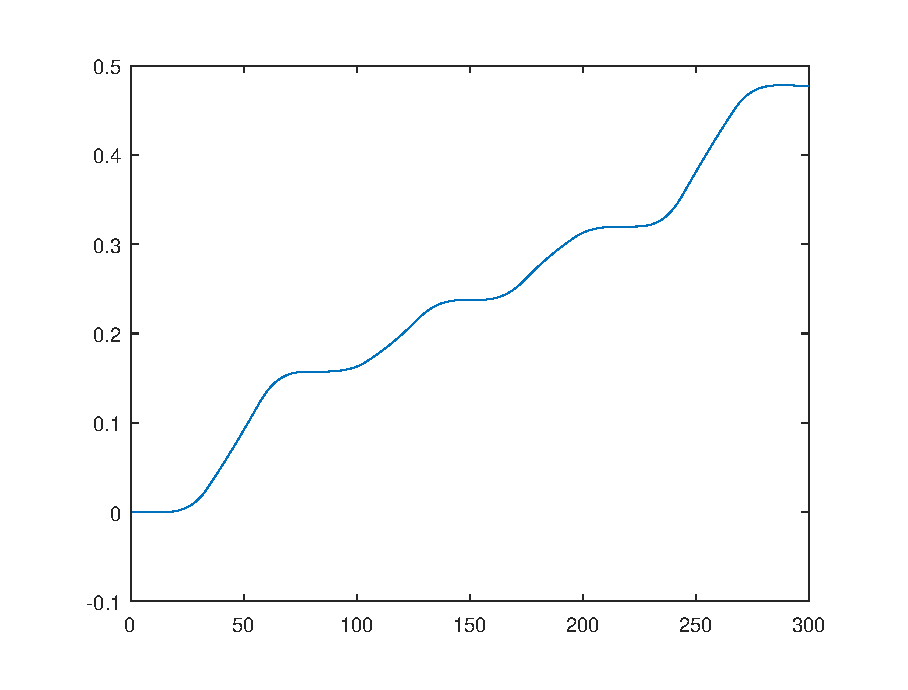
\includegraphics[width=0.5\linewidth]{img/zaxerdik}}
	\subfloat[Roll-Angle error]{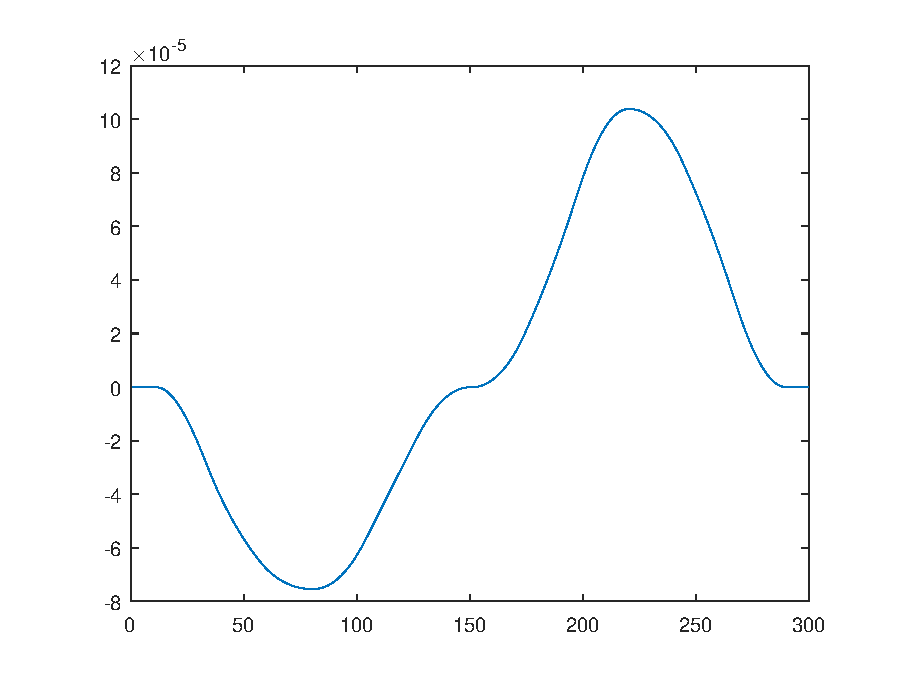
\includegraphics[width=0.5\linewidth]{img/rerdik}}
	\hspace{1cm}
	\subfloat[{Pitch-Angle error}]{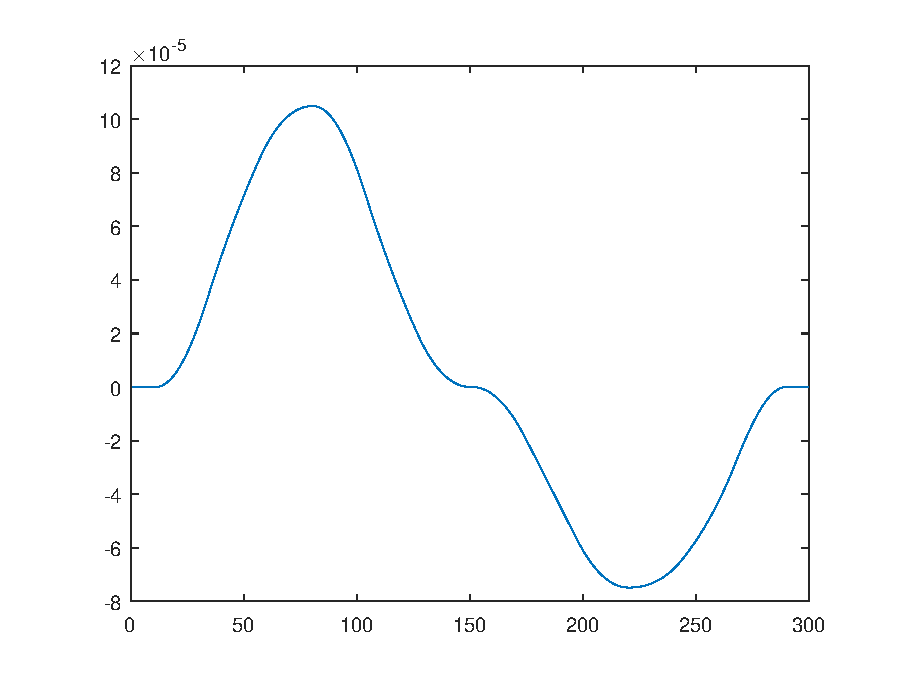
\includegraphics[width=0.5\linewidth]{img/perdik}}
	\subfloat[Manipulability]{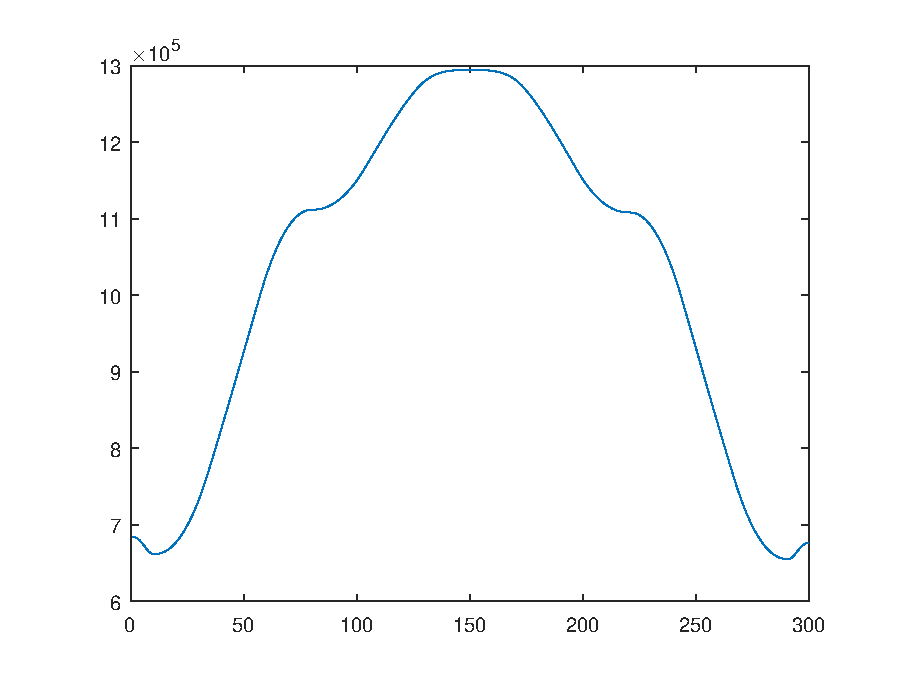
\includegraphics[width=0.5\linewidth]{img/mandik}}
	\hspace{1cm}
	\subfloat[Joint Trajectory]{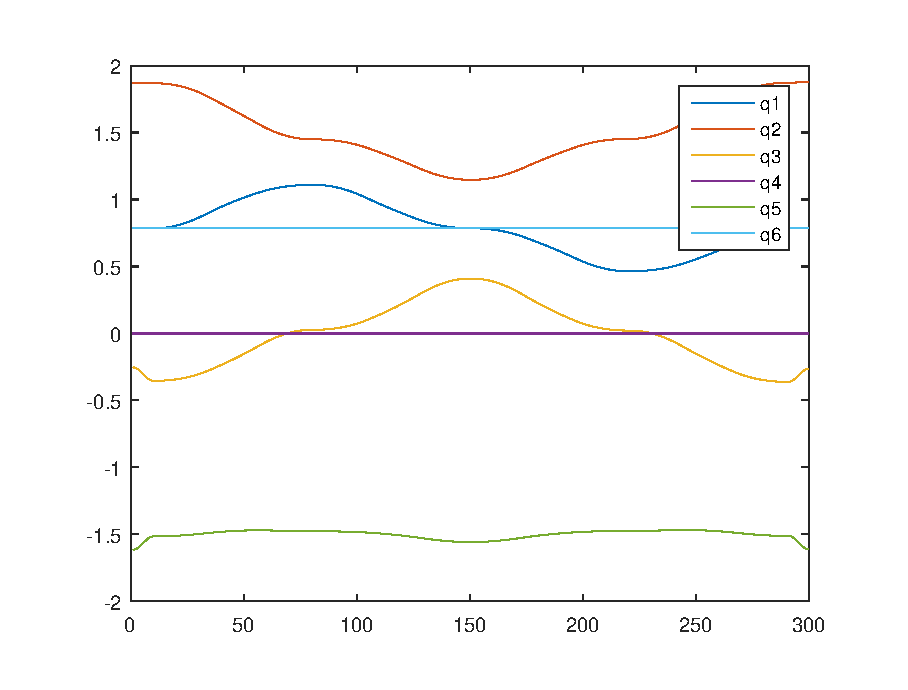
\includegraphics[width=0.5\linewidth]{img/jodik}}
\end{figure}	
\newpage
The pose error could be further reduced if the kinematics inversion is performed through the \textit{ikcon} function as described in \ref{sssec:ikcon}. In this case there are significant improvement only in the pose error while the other quantities remains almost the same and hence are not reported.
\begin{figure}[!h]
	\centering
	\subfloat[x-axes error]{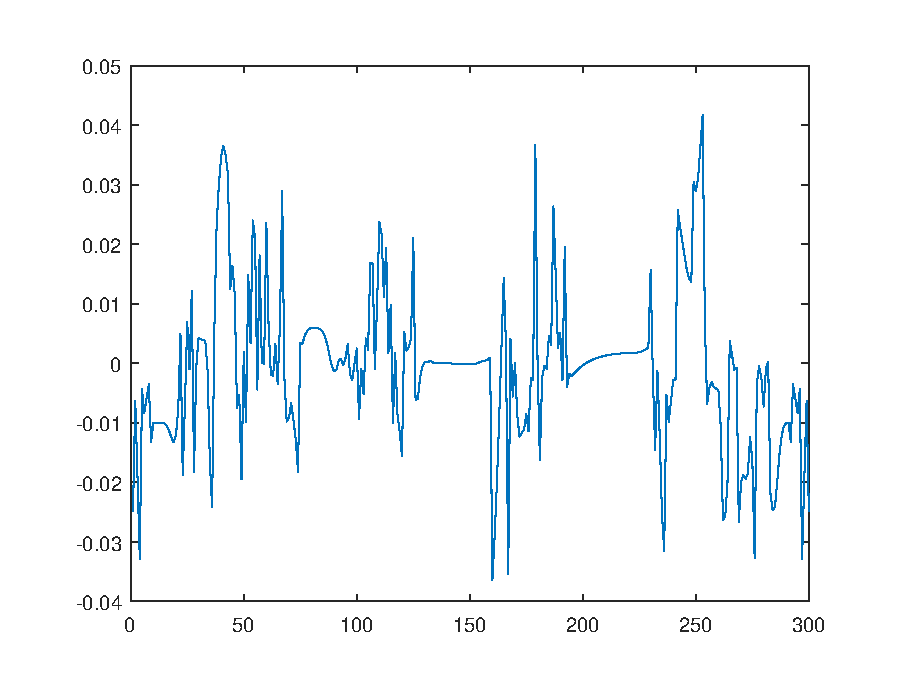
\includegraphics[width=0.5\linewidth]{img/xaxerikcon}}
	\subfloat[y-axes error]{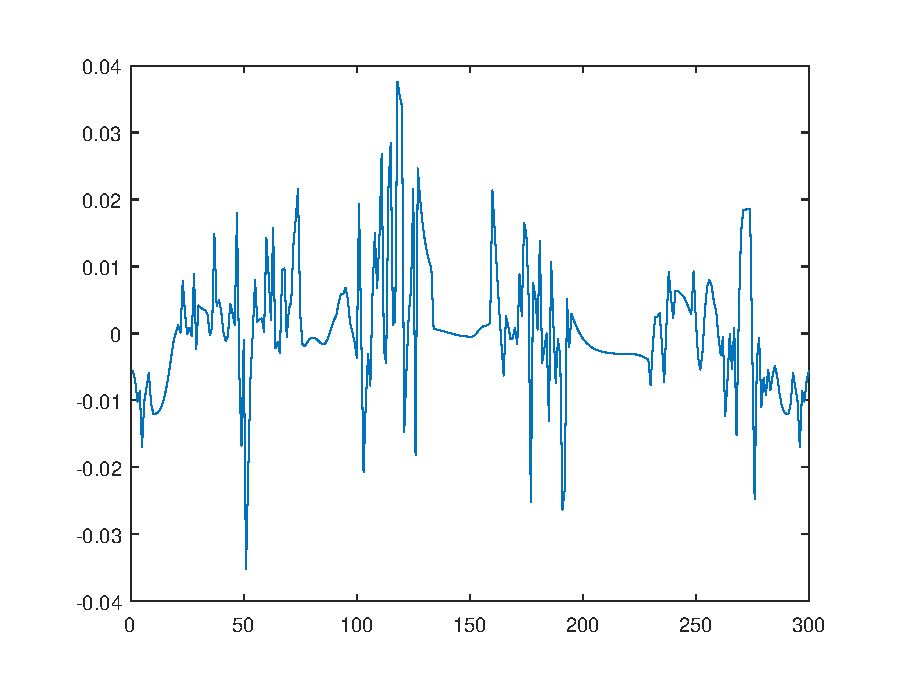
\includegraphics[width=0.5\linewidth]{img/yaxerikcon}}
	\hspace{1cm}
	\subfloat[z-axes error]{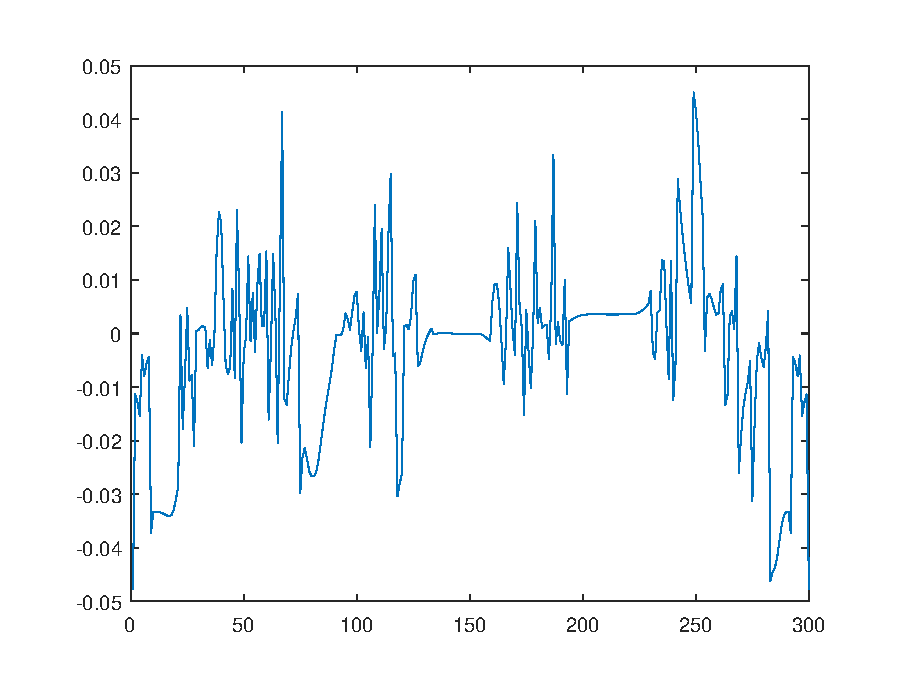
\includegraphics[width=0.5\linewidth]{img/zaxerikcon}}
\end{figure}

It is possible to see that error it's ten times less then before, such improvements has obviously a cost in terms of performance degradation due to the fact that the algorithm solves an optimization problem at each trajectory step, indeed now the whole procedure requires 8.62 seconds, i.e more than ten times the previous computation time. In this case a trade-off is necessary in order to achieve good precision in a reasonable computation time.

\subsection{Optimized Inverse Differential Kinematics}

The null-space optimization attempt to improve the manipulability measure. Fig\ref{fig:manim} shows how in average there is an improvement of $10^{-9}$ on the achieved manipulability, but in order to get this minimum results the cost paid is multiply by 100 times the computation time without it, hence in this case the optimization does not provide benefits that sufficiently counter balances the performance degradation.

\begin{figure}
	\centering
	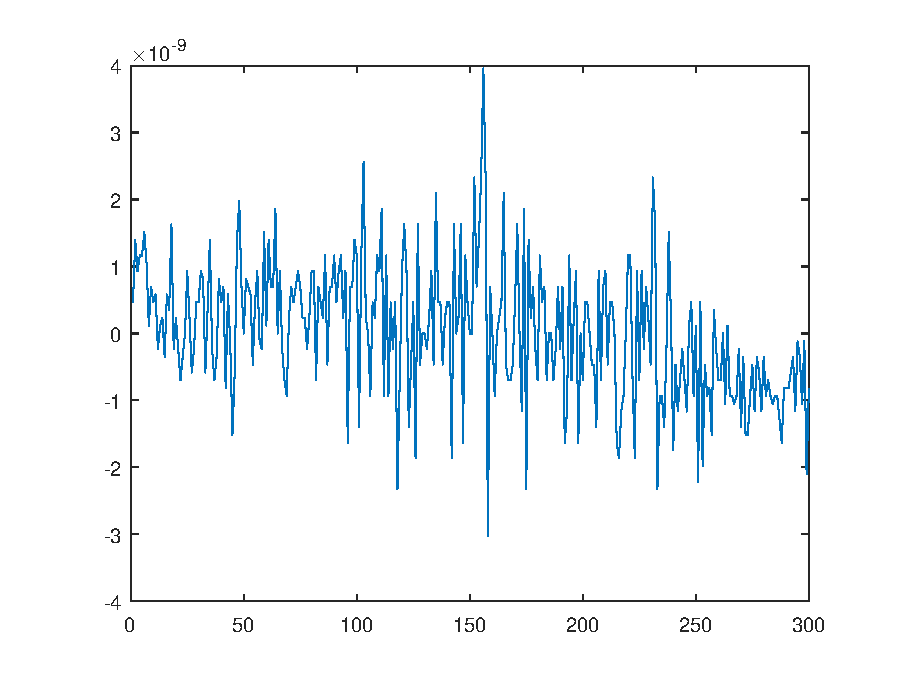
\includegraphics[width=0.8\linewidth]{img/maner}
	\caption{Manipulability improvement}
	\label{fig:manim}
\end{figure}